\documentclass{article}
\usepackage{booktabs}
\usepackage{caption}
\usepackage[margin=1in]{geometry}
\usepackage{graphicx}
\usepackage{float}
\usepackage{array}
\usepackage{siunitx}
\sisetup{scientific-notation=true}
\begin{document}
\title{Rocket Stage Optimization Report}
\author{Generated by Payload Optimization Script}
\maketitle
\section{Optimization Results}
The following table shows the optimization results for different solvers:
\begin{table}[H]
\centering
\caption{Optimization Results}
\small
\begin{tabular}{lcccc}
\toprule
\midrule
Method & Time (s) & Payload Fraction & dv & ratio \\
\midrule
SLSQP & 0.000000 & 0.031548 & [4650. 4650.] & np.float64(0.14597089895924484), np.float64(0.216125802081186) \\
differential\_evolution & 3.626201 & 0.035547 & [2772.79891319 6527.19178695] & np.float64(0.3297820716642936), np.float64(0.1077908756268375) \\
GA & 5.629594 & 0.016650 & [6866.98338561 2433.01274554] & np.float64(0.03697251531076126), np.float64(0.4503270986963582) \\
dp & 0.044316 & 0.035547 & [2771.4 6528.6] & np.float64(0.32996739307004114), np.float64(0.10772992500147) \\
\midrule
\bottomrule
\end{tabular}

\end{table}
\section{Stage Ratios}
The following table shows the stage ratios (Lambda) for each solver:
Note: Stage ratios not available in results.
\section{Input Parameters}
\subsection{Global Parameters}
The following table shows the global parameters used in the optimization:
\begin{table}[H]
\centering
\caption{Input Parameters}
\begin{tabular}{lc}
\toprule
\midrule
Parameter & Value \\
\midrule
G0 & 9.81 \\
TOTAL\_DELTA\_V & 9300 \\
\midrule
\bottomrule
\end{tabular}

\end{table}
\subsection{Stage Data}
The following table shows the parameters for each stage:
\begin{table}[H]
\centering
\caption{Stage Parameters}
\begin{tabular}{ccc}
\toprule
\midrule
stage & ISP & EPSILON \\
\midrule
1 & 300.000 & 0.060 \\
2 & 348.000 & 0.040 \\
\midrule
\bottomrule
\end{tabular}

\end{table}
\section{Visualization}
\subsection{Execution Time}
\begin{figure}[H]
\centering
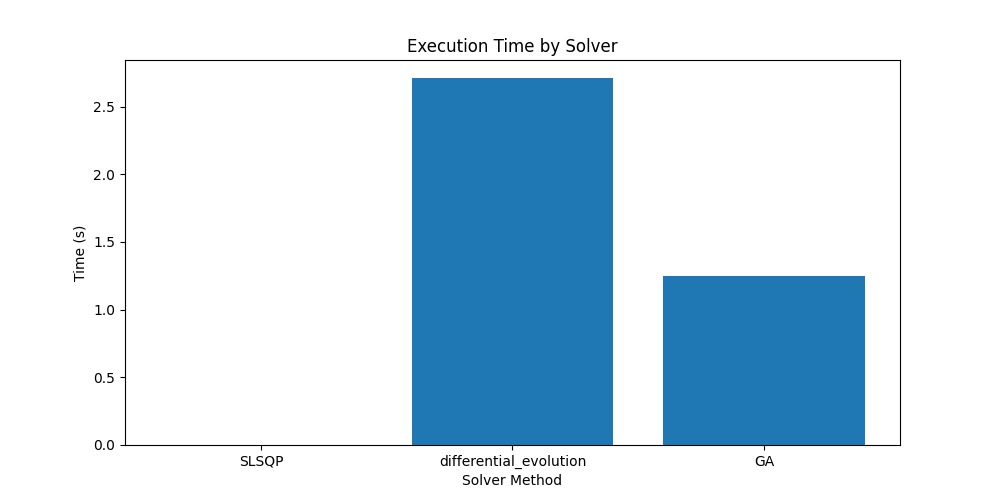
\includegraphics[width=\textwidth]{execution_time.png}
\caption{Execution time comparison between solvers}
\end{figure}
\subsection{Payload Fraction}
\begin{figure}[H]
\centering
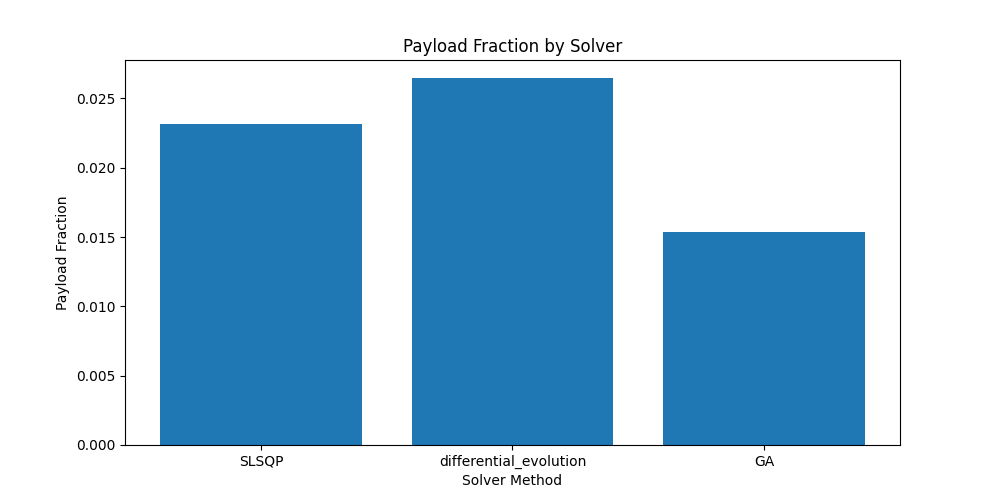
\includegraphics[width=\textwidth]{payload_fraction.png}
\caption{Payload fraction comparison between solvers}
\end{figure}
\subsection{Delta-V Breakdown}
The following figure shows the Delta-V breakdown for each solver:
\begin{figure}[H]
\centering
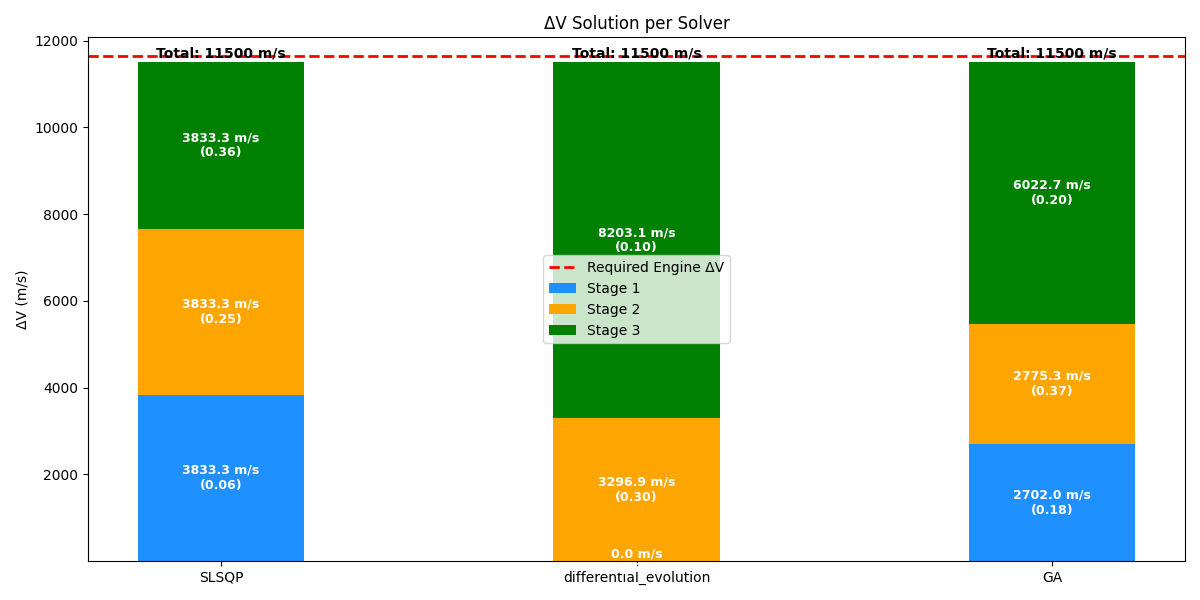
\includegraphics[width=\textwidth]{dv_breakdown.png}
\caption{Delta-V breakdown by solver}
\end{figure}
\end{document}